\documentclass{article}
\usepackage[T1]{fontenc}
\usepackage{lmodern}
\usepackage{graphicx}
\usepackage{amsmath,amssymb}
\usepackage[a4paper,margin=2cm]{geometry}
\usepackage[absolute,overlay]{textpos}
\setlength{\TPHorizModule}{1mm}
\setlength{\TPVertModule}{1mm}
\usepackage[indonesian]{babel}
\usepackage{hyperref}
\setlength{\emergencystretch}{2em}
% unit: Halaman 40

\begin{document}

% === Halaman 40 (llm) ===

\textbf{Catatan:}

\vspace{92.07mm}

\begin{enumerate}
  \item Di dalam pustaka \texttt{Crypto.PublicKey.RSA} dari \texttt{PyCryptodome}, fungsi \texttt{RSA.generate()} secara default menggunakan kunci publik $e = 0x10001$ (atau 65537 dalam desimal), karena nilai ini dianggap aman dan efisien.
  \item Namun, jika Anda ingin menspesifikasikan nilai $e$ lain (misalnya 97 atau nilai lainnya), Anda bisa menentukan nilai $e$ saat memanggil \texttt{RSA.generate()}, seperti berikut:
  
  \vspace{10mm}
  
  \item Pastikan nilai $e$ yang dipilih adalah \textbf{bilangan ganjil}, serta tidak terlalu kecil untuk menghindari potensi kelemahan RSA.
\end{enumerate}

% deskripsi: Potongan kode Python yang menunjukkan cara menggunakan PyCryptodome untuk menghasilkan kunci RSA dengan nilai e kustom.
% bbox normalisasi: [0.1900, 0.4800, 0.5600, 0.7900]
\begin{textblock*}{77.70mm}(39.90mm,142.56mm)
\noindent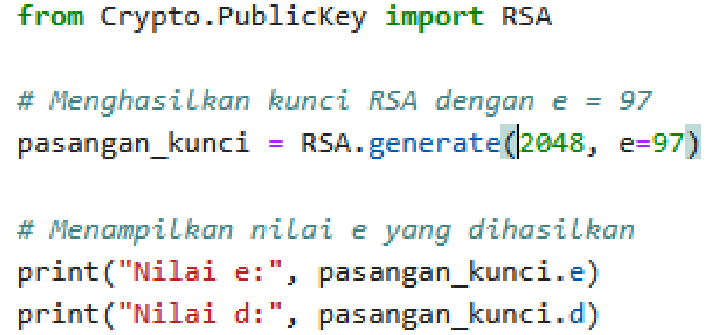
\includegraphics[width=77.70mm,height=92.07mm]{../../images/llm/page_040_img_01.png}%
\end{textblock*}

\end{document}
